\chapter{Sviluppo del progetto}
In questo capitolo verrà descritto lo scopo di questo progetto, i requisiti necessari al suo raggiungimento e i dettagli della sua struttura interna che ne permette il funzionamento. In particolare andremo ad analizzare il class-diagram che mostra le relazioni tra le classi che lo costituiscono e discuteremo delle scelte implementative fatte.

\section{Obiettivo e requisiti}
L'obiettivo di questa tesi è creare un programma che sia in grado di ricevere in ingresso la struttura del modello descritta in linguaggio XML e di scrivere in modo automatico il codice NetLogo che possa eseguire la simulazione di interesse, rendendo, quindi, trasparente il processo di scrittura del codice.\\
Il progetto è stato sviluppato in linguaggio Java. La scelta del linguaggio XML, invece, è dettata dalla sua diffusione, con lo scopo di ridurre le conoscenze preliminari necessarie per l'utilizzo di questo strumento.\\
Per l'analisi del documento XML abbiamo scelto la libreria JDOM2\footnote{http://www.jdom.org/} non inclusa in Java. Il Wold Wide Web Consortium, infatti, ha stabilito uno standard cross-platform e language-indipendent detto DOM (Document Object Model) per la rappresentazione di documenti strutturati (quindi XML, HTML, XHTML) come modello orientato agli oggetti. Il formato JDOM usato dalla libreria è una variazione dello standard disegnata appositamente per Java.\\
Lo strumento segue il seguente workflow:
\begin{itemize}
\item analisi del documento XML e costruzione di una rappresentazione della struttura orientata agli oggetti in JDOM attraverso l'omonima libreria
\item costruzione degli oggetti Java per la rappresentazione della simulazione descritta nel modello JDOM 
\item visita degli oggetti Java e scrittura su file del codice NetLogo che eseguirà la simulazione
\end{itemize}

\section{Struttura del documento XML}
La struttura del documento XML prevista per il funzionamento del nostro strumento si attiene il più possibile allo standard di formato GraphML\footnote{http://graphml.graphdrawing.org/} (approvato dal W3C) in modo da evitare inconsistenze e incomprensioni, soprattutto per la parte in cui è descritta la topologia dell'ambiente, per la quale questo formato è pienamente adatto.
Il file XML è suddiviso in tre sezioni distinte:
\begin{itemize}
\item \texttt{Graph}
\item \texttt{Behaviors}
\item \texttt{System}
\end{itemize} 
\texttt{Graph} rappresenta la topologia dell'ambiente in cui gli attori si muovono, ed è descritta sotto-forma di grafo con \texttt{edges} che rappresentano le strade e \texttt{nodes} che rappresentano gli incroci. Gli edges possono essere \texttt{directed} e \texttt{undirected}, per ognuno di essi vengono specificati peso e larghezza. I nodes invece possono essere di tre tipi, normal, entry o exit, per tutti e tre i tipi vengono specificate coordinate spaziali e dimensioni fisiche dell'incrocio che esso rappresenta.\\
Per quanto riguarda i \texttt{Behavior} si è preferito distaccarci leggermente dallo standard, in modo da avere una struttura più comprensibile, usando gli specifici tag \texttt{<behavior \textbackslash>}. Per ogni behavior viene indicato la tipologia, l'identificatore e la lista dei nodi di interesse.\\
La sezione \texttt{System} descrive lo stato iniziale (\texttt{state}) dell'ambiente. Per ogni nodo indica il numero di attori presenti e i loro behavior. In particolare nei nodi contrassegnati come entry o exit viene aggiunta una sezione denominata \texttt{parameters} in cui si specificano la frequenza di generazione o eliminazione degli attori e le percentuali relative ad ogni behavior. Per i nodi di ingresso viene anche indicato un limite superiore agli attori generabili.

\section{Class Diagram}
L'unico scopo delle classi Java utilizzate è quello di rappresentare e conservare l'informazione raccolta dal documento XML, senza eseguire alcun tipo di manipolazione. Per questo motivo abbiamo cercato di mantenere la struttura delle classi il più semplice possibile, come mostrato in Figura \ref{fig:graph-diagram}.\\
\begin{figure}[htbp]
\centering
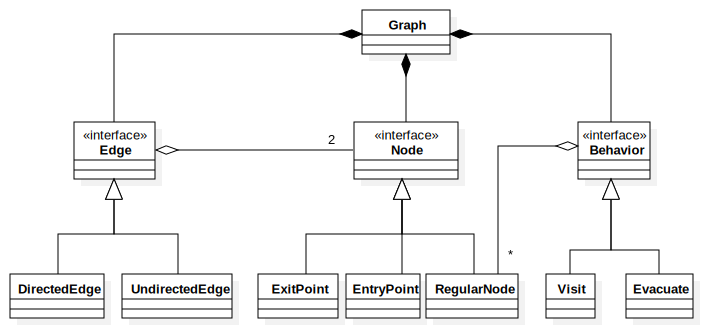
\includegraphics[width=\textwidth,height=\textheight,keepaspectratio]{images/graph-diagram.pdf}
\caption{Class diagram of the graph structure}
\label{fig:graph-diagram}
\end{figure}
Come già accennato un nodo può essere 